% mnras_template.tex
%
% LaTeX template for creating an MNRAS paper
%
% v3.0 released 14 May 2015
% (version numbers match those of mnras.cls)
%
% Copyright (C) Royal Astronomical Society 2015
% Authors:
% Keith T. Smith (Royal Astronomical Society)

% Change log
%
% v3.0 May 2015
%    Renamed to match the new package name
%    Version number matches mnras.cls
%    A few minor tweaks to wording
% v1.0 September 2013
%    Beta testing only - never publicly released
%    First version: a simple (ish) template for creating an MNRAS paper

%%%%%%%%%%%%%%%%%%%%%%%%%%%%%%%%%%%%%%%%%%%%%%%%%%
% Basic setup. Most papers should leave these options alone.
\documentclass[a4paper,fleqn,usenatbib]{mnras}

% MNRAS is set in Times font. If you don't have this installed (most LaTeX
% installations will be fine) or prefer the old Computer Modern fonts, comment
% out the following line
\usepackage{newtxtext,newtxmath}
% Depending on your LaTeX fonts installation, you might get better results with one of these:
%\usepackage{mathptmx}
%\usepackage{txfonts}

% Use vector fonts, so it zooms properly in on-screen viewing software
% Don't change these lines unless you know what you are doing
\usepackage[T1]{fontenc}
\usepackage{ae,aecompl}


%%%%% AUTHORS - PLACE YOUR OWN PACKAGES HERE %%%%%

% Only include extra packages if you really need them. Common packages are:
\usepackage{graphicx}	% Including figure files
\usepackage{amsmath}	% Advanced maths commands
\usepackage{amssymb}	% Extra maths symbols

%%%%%%%%%%%%%%%%%%%%%%%%%%%%%%%%%%%%%%%%%%%%%%%%%%

% a hack to get things to compile, see
% https://tex.stackexchange.com/questions/249579/pdfendlink-ended-up-in-different-nesting-level-than-pdfstartlink-error-with
%\usepackage{etoolbox}
%\makeatletter
%\patchcmd\@combinedblfloats{\box\@outputbox}{\unvbox\@outputbox}{}{%
%  \errmessage{\noexpand\@combinedblfloats could not be patched}%
% }%
%\makeatother

%%%%% AUTHORS - PLACE YOUR OWN COMMANDS HERE %%%%%

% Please keep new commands to a minimum, and use \newcommand not \def to avoid
% overwriting existing commands. Example:
%\newcommand{\pcm}{\,cm$^{-2}$}	% per cm-squared

%%%%%%%%%%%%%%%%%%%%%%%%%%%%%%%%%%%%%%%%%%%%%%%%%%

%%%%%%%%%%%%%%%%%%% TITLE PAGE %%%%%%%%%%%%%%%%%%%

% Title of the paper, and the short title which is used in the headers.
% Keep the title short and informative.
\title[Infrared excesses of HD~116434 and 51 Eri]{Faint circumstellar
  emission in directly imaged planet systems: \\ The infrared excesses
  of HD~116434 and 51~Eri.}

% The list of authors, and the short list which is used in the headers.
% If you need two or more lines of authors, add an extra line using \newauthor
\author[G. M Kennedy]{
Grant M. Kennedy$^{1}$\thanks{E-mail: gkennedy@ast.cam.ac.uk}
\\
% List of institutions
$^{1}$Institute of Astronomy, University of Cambridge, Madingley Road, Cambridge CB3
  0HA, UK 
}

% These dates will be filled out by the publisher
\date{Accepted XXX. Received YYY; in original form ZZZ}

% Enter the current year, for the copyright statements etc.
\pubyear{2017}

% Don't change these lines
\begin{document}
\label{firstpage}
\pagerange{\pageref{firstpage}--\pageref{lastpage}}
\maketitle

% Abstract of the paper
\begin{abstract}
  The high rate of infrared excess detections towards stars discovered
  to host wide-orbit planets by direct imaging is intriguing, as it may
  provide a link between planets and planetesimal belts (the ``debris
  disks''), and thus key information about how these systems
  formed. This correlation is 2-3$\sigma$ significant for A and F-type
  host systems, but only if the bias towards observing excess systems in
  search of these planets is ignored, so awaits future work that uses an
  unbiased sample.  The possible existence of this trend motivates
  careful searches for infrared excesses in all systems with directly
  imaged planets, and consideration of the planetary system architecture
  in each case. Here the system HD~116434, host to a planet at a
  projected separation of 92au, is reconsidered, and shown to have a
  4$\sigma$ significant 24$\mu$m excess that must originate interior to
  the orbit of HD~116434~b. JWST and ALMA follow-up is encouraged to
  confirm the excess, and test the possibility that it originates from
  Be star-like stellar wind emission rather than a debris disk. The disk
  around 51~Eridani is also reconsidered; a synthesis of previous
  results finds that only a single temperature component is needed to
  model the disk spectrum, and that the location of this belt relative
  to the planet (projected separation of 13au) is unclear. When dust
  optical properties and collisional evolution are considered, the most
  probable location is exterior to the planet 51~Eri~b. Thus, while
  conclusions on the planet-disk correlation await a detailed and
  unbiased sample analysis, work in the meantime remains inspired by the
  diverse nature and architectures of individual systems with directly
  imaged planets.
\end{abstract}

% Select between one and six entries from the list of approved keywords.
% Don't make up new ones.
\begin{keywords}
  planets and satellites: general -- planet-disc interactions --
  planetary systems -- circumstellar matter -- stars:individual:
  HD~116434 -- stars:individual: 51 Eridani
\end{keywords}

%%%%%%%%%%%%%%%%%%%%%%%%%%%%%%%%%%%%%%%%%%%%%%%%%%

%%%%%%%%%%%%%%%%% BODY OF PAPER %%%%%%%%%%%%%%%%%%

\section{Introduction}

One of the most profound insights into planet formation comes from
noting the prograde and near-coplanar orbits of the Solar System's
planets; any theory of their formation will conclude that they formed in
a disk that orbited the young Sun. Further insight comes from the
objects captured into exterior resonances with Neptune; the existence of
these objects leads to the conclusion that Neptune was previously closer
to the Sun, and captured these objects during a period of outward
migration \citep{1993Natur.365..819M}.

The state of our understanding of analogous processes around other stars
lies somewhere between these cases. It is clear that most other stars
host disks when they are young \citep[e.g.][]{2001ApJ...553L.153H}, and
while the typical outcomes are different to the Solar System, planet
formation tends to yield systems that are consistent with having formed
in a disk \citep[e.g.][]{2012Natur.487..449S}. What is unclear however,
is how planets and disks are related on a system-by-system basis. How
are the properties of a given planet related to those of the gas-rich
disk in which it forms, or to the gas-poor disk of planetesimals --
the ``debris disk'' -- that orbits the same star on the main-sequence?

Finding links between primordial disks and planets is hard, simply
because these disks are optically thick, so planets must be very massive
to repel gas from their orbital regions and thus be detectable
\citep[e.g.][]{2007prpl.conf..655P}. Lower-mass planets may reveal their
presence via their influence on the disk, but unless these planets are
detected, whether observed disk structures truly owe their existence to
unseen planets can be debatable
\citep{2015ApJ...813...88Z,2017ApJ...839L..24M}.

Around older stars, empirical evidence is emerging that disks and planet
properties are related; Herschel observations find that debris disks
tend to be brighter in systems that host radial velocity-detected
planets \citep{2013AAS...22114424B,2015ESS.....312014B}. Similarly,
evidence for a similar trend appears to be emerging in systems with
directly imaged planets; of the six systems with A/F-type host stars
\citep[HR~8799, Fomalhaut, $\beta$ Pictoris, HD~95086, HD~106906,
51~Eri,][]{2008Sci...322.1348M,2008Sci...322.1345K,2010Sci...329...57L,2013ApJ...772L..15R,2014ApJ...780L...4B,2015Sci...350...64M},\footnote{HD~131399,
  a system for which a disk has not been detected, is excluded from this
  list as it is currently unclear whether the object discovered by
  \citet{2016Sci...353..673W} is planet orbiting in this system, see
  \citet{2017arXiv170506851N}. If the object is a planet in this system,
  this system might alternatively be excluded as a binary with a
  relatively small separation ($\sim$300au).} all have significant
infrared excesses originating from debris disks
\citep{1984Sci...226.1421S,1985PASP...97..885A,2005ApJ...623..493C,2006ApJS..166..351C,2009ApJ...705..314S,2014ApJS..212...10P,2014A&A...565A..68R}. The
possibility of a correlation provides motivation for detailed scrutiny
of every system discovered to host a directly imaged planet, and of
control samples, as these conclusions will be key for the significance
or otherwise of any trend.

This paper is motivated by the recent discovery of a planet orbiting the
star HD~116434 \citep{2017arXiv170701413C}. Whether this star shows an
infrared excess is unclear, earlier work found a 3.5$\sigma$ excess at
24$\mu$m, but conservatively required 6$\sigma$ for an excess to be
considered robust
\citep{2012ApJ...756..133C}. \citet{2017arXiv170701413C} briefly
revisited this work, giving limits on the level of undetected cool dust
emission. Here, the conclusion for this system is revisited in detail in
section \ref{s:hd116434}. A significant excess is found, and the
possible nature of this excess and the architecture of the planetary
system is then discussed. The system 51~Eri also hosts a faint (but
robust) excess, but the reported properties of the disk around this star
are inconsistent, so this system (including the companion GJ~3305~AB),
is revisited in section \ref{s:51eri}. We briefly consider the
correlation between debris disk brightness and the detection of directly
imaged planets around A and F-type stars in section \ref{s:corr}, and
conclude in section \ref{s:conc}.

\section{Revisiting the infrared excess of HD~116434}\label{s:hd116434}

\subsection{Previous infrared excess studies}\label{s:hd116434:ss:prev}

Two previous works have considered infrared observations of HD~116434
and whether this star shows an infrared
excess. \cite{2012MNRAS.427..343M} used all-sky data from AKARI
\citep{2010A&A...514A...1I} and the Wide-field Infrared Explorer
\citep[WISE,][]{2010AJ....140.1868W} to consider $\sim$10$^5$ stars in
the Hipparcos catalogue, deriving stellar parameters and looking for
infrared excesses. For HD~116434 their catalogue has fractional excesses
(the observed to photospheric flux density ratio)
$R_{\rm obs} = F_{\rm obs}/P_{\rm obs}$ of 1.12, 1.05, and 1.14 at 9,
12, and 22$\mu$m, deriving a fractional luminosity
$L_{\rm disk}/L_\star$ of $2 \times 10^{-4}$. However, they do not
consider the statistical significance of their excesses, nor do they
specifically discuss HD~116434 (the focus of their work being largely on
giant stars, rather than dwarfs).

\citet{2012ApJ...756..133C} used the Multiband Imaging Photometer for
\emph{Spitzer} \citep[MIPS,][]{2004ApJS..154....1W,2004ApJS..154...25R}
to survey 216 B and A-type stars in Scorpius-Centaurus at 24 and
70$\mu$m, with HD~116434 part of their Lower Centaurus Crux (LCC)
sub-sample. At 70$\mu$m they reported a 3$\sigma$ upper limit of
11.4mJy. They derived excesses at 24$\mu$m using the $K_s - [24]$ colour
relation, and estimated their significance as
$\chi_{\rm obs} = [F_{\rm obs}-P_{\rm obs}]/\sigma$, where $\sigma$
includes uncertainty contributions from both $K_s$ and 24$\mu$m
photometry. They set $\chi_{24} > 6$ their criterion for an excess,
which meant that while HD~116434 was found to have $\chi_{24} = 3.5$, a
value large enough to warrant suspicion of an excess, they did not
consider excesses at this level formally significant. Inspection of the
distribution of $\chi_{24}$ in their Figure 2 suggests that setting a
criterion of 6 was conservative, and that a lower threshold could
probably have been justified.

\citet{2017arXiv170701413C} did not carry out a re-analysis of infrared
observations, but used the MIPS 70$\mu$m upper limit and WISE 22$\mu$m
observation (assuming no excess) to set limits on the dust levels as a
function of stellocentric radius.

Thus, two previous works provide evidence that HD~116434 may show a weak
mid-infrared excess. Given the aforementioned importance of excesses in
systems with directly imaged planets, the robustness of the 24$\mu$m
excess is now revisited within the context of a population of B and
A-type stars in Scorpius-Centaurus.

\subsection{Detection}\label{s:hd116434:ss:det}

\begin{figure*}
  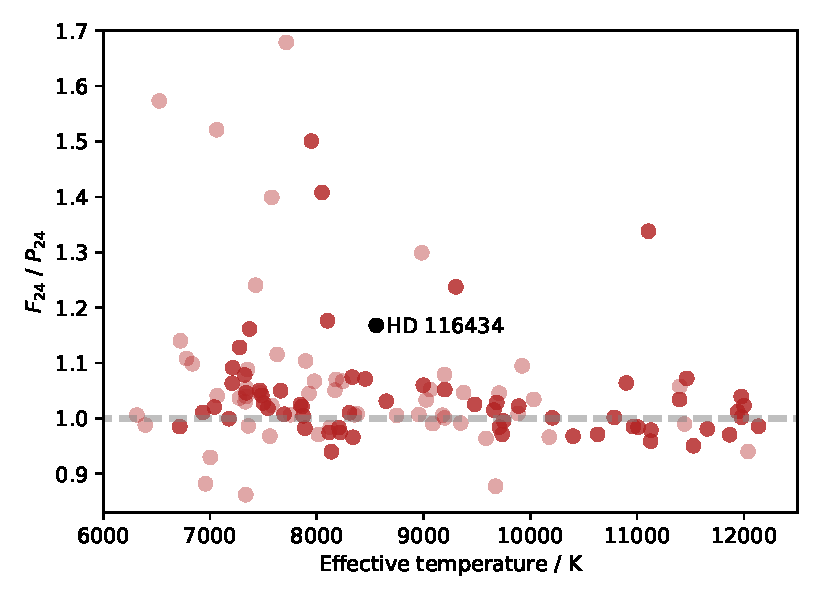
\includegraphics[width=\columnwidth]{r_Teff.pdf}
  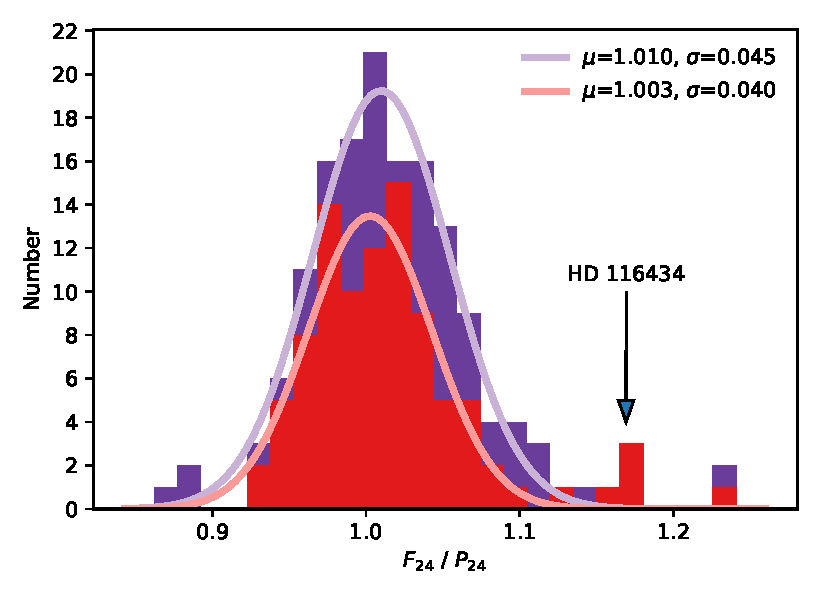
\includegraphics[width=\columnwidth]{r.pdf}
  \caption{$F_{24}/P_{24}$ distributions for the Sco Cen
    sample. (\emph{left panel}) The distribution as a function of
    $T_{\rm eff}$ (dark dots, up to $T_{\rm eff}=12,500$K), with
    HD~116434 noted by the black dot. Light dots indicate sources
    flagged as having potential background contamination. (\emph{right
      panel} Histograms for all targets (blue bars) and those with
    uncontaminated images (red bars). Targets above 12,500K are
    included. Lines show corresponding Gaussian fits to each population,
    with mean and standard deviation given by the legend. The location
    of HD~116434 is marked by the arrow.}
    \label{fig:r}
\end{figure*}

This section quantifies the significance of any excess at 24$\mu$m in
HD~116434's spectrum. Photometry from the \emph{Spitzer} Enhanced
Imaging Products (SEIP) was used at 24$\mu$m, along with data from the
Wide-field Infrared Explorer \citep[WISE,][]{2010AJ....140.1868W}, AKARI
\citep{2010A&A...514A...1I}, 2MASS \citep{2006AJ....131.1163S},
Hipparcos/Tycho-2 \citep{1997ESASP1200.....P}, and a range of other
optical literature sources.\footnote{Details are given in the Appendix,
  and all data used in this work are available online. The model fitting
  method is that used in previous works
  \citep[e.g.][]{2014MNRAS.445.2558T,2012MNRAS.426...91K,2014MNRAS.444.3164K,2017RSOS....460652K},
  but with updated software that is available at
  \href{https://github.com/drgmk}{github.com/drgmk} (as are the results
  from this paper). Proof that this method is robust is given by the
  fact that the photospheric predictions are precise enough to detect
  the excess around HD~116434.}  A fit to the flux density distribution
(commonly called the spectral energy distribution or SED), of HD~116434
yields an excess detection at 24$\mu$m. The MIPS point is a 4$\sigma$
outlier in the residuals, implying that the spectrum is not well
modelled by a single stellar photosphere. While this star was observed
by WISE, this photometry is not as precise, and is only 2$\sigma$ above
the photospheric model. A likely conclusion is therefore that an
infrared excess is present, which given a lack of excess at shorter
wavelengths, which for a main-sequence A-type stars would normally be
taken as evidence for a debris disk.

However, this result in isolation does not tell the whole story. The
MIPS photometry could actually be much worse than indicated by the
uncertainties given by the SEIP, in which case the 4$\sigma$ excess is
simply the result of a small positive offset in the 24$\mu$m data for
HD~116434 and unrealistically optimistic error estimation. The usual way
to address this issue is to investigate the excess properties for a
population of targets \citep[e.g.][]{2006ApJ...653..675S}. While the
distribution may be studied empirically (e.g. using colours such as
$K_s - [24]$), here photospheric modelling is done for all targets,
using only photometry at wavelengths shorter than 20$\mu$m, and the
predictions $P_{24}$ of the models compared to the data $F_{24}$. z

The results of this procedure, as applied to the Sco-Cen targets in
\citet{2012ApJ...756..133C}, are shown in Figure \ref{fig:r}. Because we
use the SEIP, some targets in fields with high cirrus levels are not
robustly detected in this catalogue, leaving 200 of 216 with 24$\mu$m
photometry. The left panel shows the distribution of
$R_{24}=F_{24}/P_{24}$ as a function of fitted stellar effective
temperature for $T_{\rm eff}<12,000$K, and the right panel shows
histograms of this distribution for all $T_{\rm eff}$ (up to 19,000K),
including and excluding targets whose MIPS images show high background
levels \citep[as flagged by][noting that HD~116434 itself was not
flagged]{2012ApJ...756..133C}.

The left panel of Figure \ref{fig:r} shows a tight distribution of
$R_{24}$ near 1, as would be expected for stars that are well modelled
as pure photospheres, plus a handful of targets with $R_{24}$ well above
this distribution \citep[some are above the plotted range, see][for a
thorough discussion of the population
properties]{2012ApJ...756..133C}. Our target of interest, HD~116434, is
clearly separated from the $R_{24} \approx 1$ population in the left
panel.

Whether this separation is statistically significant is addressed by the
right panel of Figure \ref{fig:r}, which shows Gaussian fits to the
entire $R_{24}$ distribution, and to the subset that do not have high
background levels. The reason for using the whole sample of B/A stars
here is that the fraction of A-type stars with excesses is rather high,
about 33\%, but much lower for the B-types (5\%). Thus, the scatter
about $R_{24}=1$ for B-types provides a good estimate of the accuracy
and precision of the 24$\mu$m predictions, and reduces the influence of
low-level excesses around the A-types when fitting the Gaussians.

The right panel shows that HD~116434, with $R_{24}=1.17$, is indeed
significantly above the bulk population, at a level of 4$\sigma$ when
possibly suspect photometry is excluded. Thus, the conclusion from this
self-calibrated population analysis is that HD~116434 does indeed show a
significant excess at 24$\mu$m. Perhaps surprisingly, this level of
significance is only slightly higher than reached by
\citet{2012ApJ...756..133C}, but they did not consider this level to be
enough to warrant a true excess. This in no way detracts from their
analysis, but simply reflects that their approach was more conservative
than the present one, which is inspired by the desire to know in detail
the properties of one specific target.

\subsection{Properties}\label{s:hd116434:ss:prop}

\begin{figure*}
  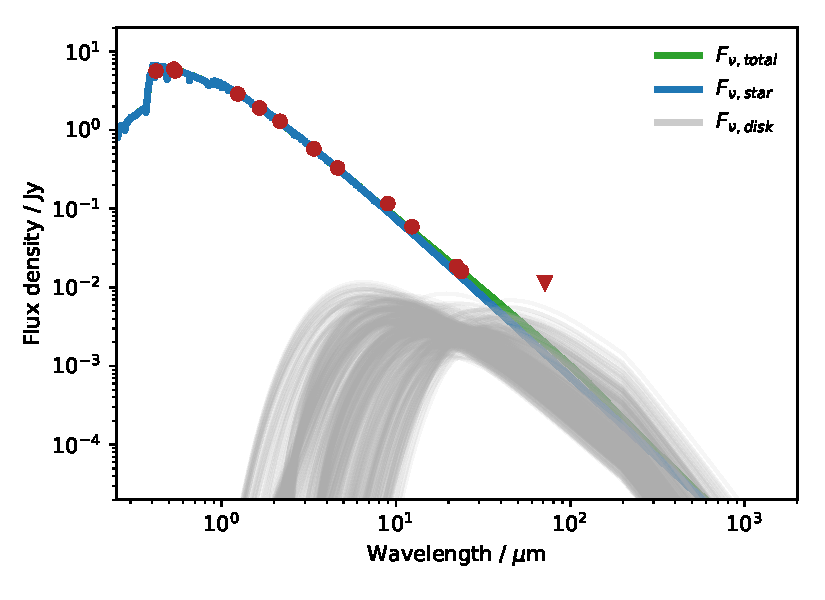
\includegraphics[width=\columnwidth]{sed.pdf}
  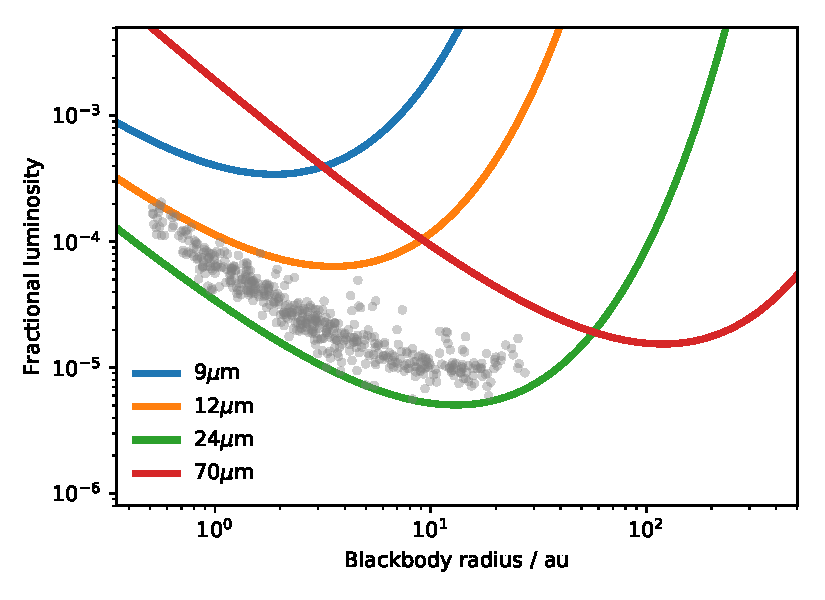
\includegraphics[width=\columnwidth]{f_r.pdf}
  \caption{Possible spectra of blackbody dust disk emission around
    HD~116434. (\emph{left panel}) Spectrum of the star (blue line) and
    photometry (dots and triangle), with possible disk realisations from
    the MCMC run (grey lines). (\emph{right panel}) Fractional
    luminosity vs. blackbody dust radius, with the 3$\sigma$ detection
    limits that are achieved with these data (solid lines) and the same
    disk realisations as the left panel (dots).}
    \label{fig:sed}
\end{figure*}

Given the likelihood of a detectable infrared excess for HD~116434, it
is of course important to understand the properties of said exces, and
how it relates to the planet at a projected separation of 92au. With a
detection at only a single wavelength, the temperature of the emission
is not well constrained, but is limited by a lack of excess at
wavelengths shorter than 24$\mu$m, and the non-detection at 70$\mu$m.

Assuming that the emission has a blackbody emission spectrum, as is
typical for dust in debris disks, the distribution of allowed
temperatures is found using a Markov-Chain Mote-Carlo (MCMC) approach,
using the \texttt{emcee} package
\citep{gw2010,2013PASP..125..306F}. Starting from the best-fit
parameters, 500 walkers were run for 1,000 steps to allow the chains to
spread throughout the allowed parameter space, and the left panel of
Figure \ref{fig:sed} shows the final states of these 500 walkers. That
is, the grey lines show 500 possible realisations of the blackbody
properties, and the fact that there are more warm curves than cool
curves implies that any emission around HD~116434 is more likely to be
warmer than cooler. The preference for warmer emission arises partially
because of the 70$\mu$m upper limit, but in addition the WISE 2$\sigma$
excess at 22$\mu$m disfavours cooler temperatures.

The right panel of Figure \ref{fig:sed} shows these temperatures
converted into stellocentric dust radii assuming blackbody properties,
and the corresponding fractional luminosities $f=L_{\rm
  disk}/L_\star$. Also shown are approximate detection limits at 9, 12,
24, and 70$\mu$m, where the uncertainties that set these limits is the
quadrature sum of the observed and photometric errors
\citep[see][]{2008ARA&A..46..339W}.

The dots illustrate the range of possible blackbody radii for the dust,
which vary from about 0.5 to 30au (800 to 100K). Thus, if the dust
particles behave like blackbodies the dust must lie interior to the
planet HD~116434 b. It is well known however from comparison of spectra
and resolved imaging that the dust in debris disks tends to be hotter
than expected for a blackbody
\citep[e.g.][]{2012ApJ...745..147R,2013MNRAS.428.1263B,2016ApJ...831...97M},
meaning that disk radii can be several times larger than blackbody
estimates. In the case of A-type stars such as HD~116434, this factor is
somewhere between 1-2, meaning that the dust here should lie at a
stellocentric distance no greater than about 60au, and that the
conclusion that the dust lies interior to the planet is robust.

The lines in Figure \ref{fig:sed} show what can be ruled out given the
data, where disks of a given fractional luminosity can be detected at a
given wavelength if they lie above the lines. The dots lie above only
the 24$\mu$m line because the excess is only detected at this
wavelength, and are bounded by non-detections at 12 and 70$\mu$m. That
the dots also lie below the 9$\mu$m (AKARI/IRC) line suggests that the
$f=2 \times 10^{-4}$ excess near this wavelength reported by
\citet{2012MNRAS.427..343M} is unlikely to have been
significant. Finally, the 70$\mu$m line rules out disks that could orbit
beyond HD~116434~b, as long as those disks have
$f \gtrsim 2 \times 10^{-5}$.

Thus far the analysis has assumed that the emission spectrum that causes
the excess can be modelled as a blackbody, as would originate in a
circumstellar debris disk. However, the very high rotation rate of
HD~116434, and the warm to hot temperatures derived for the disk
temperature, are reminiscent of the infrared excesses originating in
free-free emission seen towards Be stars
\citep{1970A&A.....9..252W,1974ApJ...191..675G}. \citet{2017arXiv170701413C}
also note the possibility that HD~116434 shows variability that might be
attributed to pulsations, another property of Be stars. This free-free
emission is typically a power law with
$F_{\rm nu} \propto \lambda^{-0.6}$, but when observed over a short
wavelength range can be fit reasonably well with a blackbody. Thus, it
seems possible that HD~116434 does not actually host a debris disk, but
is instead driving a stellar wind \citep[estimated to be
$10^{-8} M_\odot$ year$^{-1}$ using eq (24) from ][the same as estimated
for Fomalhaut by \citet{2012A&A...540A.125A}]{1975A&A....39....1P}. The
excesses seen towards main-sequence Be stars in debris disk surveys tend
to be much larger than seen here however
\citep[e.g.][]{2006ApJ...653..675S,2012ApJ...756..133C}, which might be
the consequence of a weaker wind from a later type star. Be stars are
normally identified by Balmer line emission in their spectra, but none
were reported by \citet{2017arXiv170701413C} for HD~116434. However,
because they originate in the same region, the strength of the H$\alpha$
line flux is known to correlate with the infrared excess
\citep{1982MNRAS.198..659N}, so a non-detection of H$\alpha$ emission
for HD~116434 may be consistent with the weak infrared emission.

Regardless of the origin, it is clear that the excess reported here is
at the limits of detection, so should be confirmed or rejected with new
observations. If the excess originates from a wind, a clear prediction
is that an excess should be easily detectable at millimeter wavelengths,
for example with ALMA; the extrapolated flux assuming a free-free
emission spectrum $\propto \lambda^{-0.6}$ is about 240$\mu$Jy at 1mm,
and should originate from a compact region around the star (within a few
au). If the excess emission is from circumstellar dust however, Figure
\ref{fig:sed} shows that an ALMA detection will be difficult, and that
non-detection will not rule out the existence of a disk with the
properties given above.

In terms of scattered light form a debris disk, the dots in Figure
\ref{fig:sed} shows that unless the disk is small, it has a low
fractional luminosity at levels of about $10^{-5}$, which is much lower
than normally required for detection, though may be aided if the high
rotational velocity indicates an edge-on disk. Conversely, for the disk
to have a high fractional luminosity it must be small, which is again a
challenge for resolved imaging.

Mid-infrared observations that in essence repeat the MIPS 24$\mu$m
detection will be the most useful, for which the only instrument
available will be the Mid-InfraRed Instrument (MIRI) on the James Webb
Space Telescope
\citep[JWST,][]{2015PASP..127..584R,2015PASP..127..612B,2015PASP..127..646W}. The
uncertainties in the disk spatial scale means that even the success of
resolved JWST imaging will be uncertain. The allowed temperatures for
the HD~116434 disk constrain it to lie well with 100au, meaning that it
is no more than 2\arcsec~in diameter, and could be significantly
smaller, especially if excess originates in a stellar wind . Disk
imaging with MIRI, which has spatial resolution of about 0.8\arcsec~at
23$\mu$m, will therefore be challenging, but with high quality
photometric calibration should still yield an excess.

The departure from a Rayleigh-Jeans slope should however be detectable
with the Medium Resolution Spectrometer, and may show silicate spectral
features that yield the dust grain size and composition, or hydrogen
emission lines in the case of a stellar wind. Thus, ALMA observations
and a mid-infrared spectrum are the most obvious and pressing
observation to i) establish the existence or otherwise of the excess,
and ii) provide insight into its origin.

\section{Revisiting the disk around 51~Eri}\label{s:51eri}

While neither its existence or nature are in doubt, the disk around
51~Eri also suffers from poor spectral characterisation, and the same
question of the disk location with respect to the planet again
arises. In this section the disk spectrum is considered in much the same
way as for HD~116434. The difference is that 51~Eri is well-known to
have an infrared excess that has previously been detected at several
wavelengths \citep{2014ApJS..212...10P,2014A&A...565A..68R}, which have
been taken to independently indicate the presence of dust orbiting both
interior and exterior to 51~Eri~b \citep{2015Sci...350...64M}. These
detections have however not been synthesised in drawing conclusions on
the probable properties of the disk, and the location relative to
51~Eri~b

\subsection{Previous infrared excess studies}\label{s:51eri:ss:prev}

Two studies have detected IR excess emission in the spectrum of 51~Eri
\citep{2014ApJS..212...10P,2014A&A...565A..68R}. Prior attempts were
unsuccessful, largely due to a lack of sensitivity, though it appears
that the MIPS 24 $\mu$m photometry presented in
\citet{2008ApJ...681.1484R} that was consistent with the photospheric
flux of 114 mJy was either more uncertain than their estimated 4\%
systematic uncertainty, or the measurement was underestimated. Updated
MIPS photometry from the SEIP finds a flux of $129.7 \pm 1$ mJy,
significantly (3$\sigma$) higher than their $115 \pm 4.6$
mJy. \cite{2014ApJS..212...10P} found 51~Eri to have a clear
(3.76$\sigma$) WISE 22 $\mu$m excess based on the 12-22 $\mu$m colour (a
22 $\mu$m flux of $146 \pm 3$ mJy compared to the photosphere of 129
mJy, where the difference compared to MIPS at 24$\mu$m is almost
certainly due to the slightly shorter wavelength). Though they quoted a
temperature of 179K based on the 12 and 22 $\mu$m photometry, this
single band excess did not constrain the dust temperature and they in
fact set an upper limit of 344K. \citet{2014A&A...565A..68R} found
51~Eri to have significant excesses at 70 and 100 $\mu$m using
\emph{Herschel} PACS \citep{2010A&A...518L...1P,2010A&A...518L...2P},
with the dust emission consistent with a temperature of 50K, albeit with
a considerable uncertainty ($\pm$20K).

While these two conclusions do not appear contradictory they are not
based on the same information, and require dust emission from at least
two components with different dust temperatures, and presumably led
\citet{2015Sci...350...64M} to conclude that 51~Eri hosts multiple
debris belts. The reason is that the 50K component derived from the PACS
photometry produces no significant emission at 22 $\mu$m. However, it is
almost certain that the upper constraint on the temperature of 70K
(1$\sigma$) arises because the SED model of \citet{2014A&A...565A..68R}
used the \citet{2008ApJ...681.1484R} photometry and therefore
\emph{required} the dust emission at 24 $\mu$m to be negligible. An
additional issue is that at such a cool temperature the dust might be
sufficiently far from the star for the disk to be resolved with PACS,
with resolution of 6-7\arcsec. That is, 50K corresponds to 74 au (a
2.5\arcsec~radius) for blackbodies around 51~Eri, and as noted above
disk sizes tend to be $\sim$1-2 times larger than the blackbody size for
early-type stars.

The constraint of $<$344K based on the 22 $\mu$m excess is not
inconsistent with the PACS detection however. Thus, the question is
whether reconsideration of the PACS data using the 22 $\mu$m flux from
WISE, and the updated MIPS 24 $\mu$m flux, leads to the same conclusion
of multiple temperature components, or if a single component will
suffice. This question would of course be rather uninteresting if it
were not for the existence of the planet 51~Eri~b, which resides at a
distance that would likely place it in between the two putative disk
components, as is seen for $\beta$ Pic, HR~8799, and HD~95086.

\subsection{Properties}\label{s:51eri:ss:prop}

\begin{figure*}
  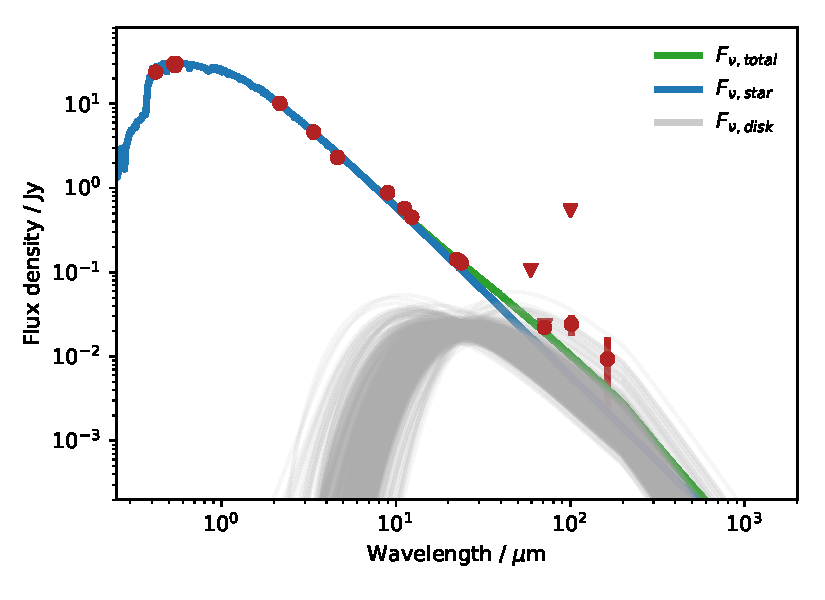
\includegraphics[width=\columnwidth]{sed_51eri.pdf}
  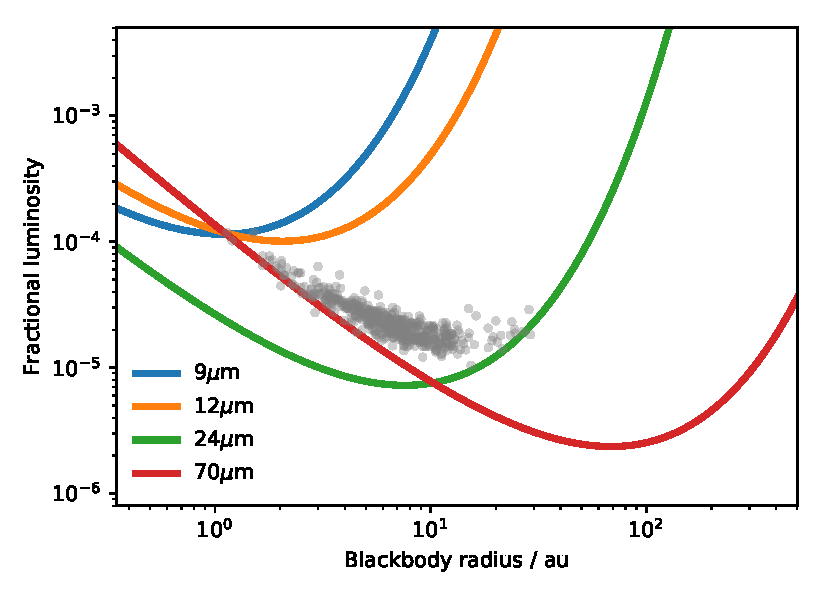
\includegraphics[width=\columnwidth]{f_r_51eri.pdf}
  \caption{Possible spectra of the disk around 51~Eri. (\emph{left
      panel}) Spectrum of the star (blue line) and photometry (dots and
    triangle), with possible disk realisations from the MCMC run (grey
    lines). (\emph{right panel}) Fractional luminosity vs. blackbody
    dust radius, with the 3$\sigma$ detection limits that are achieved
    at 12, 24 and 70$\mu$m (solid lines) and the same disk realisations
    as the left panel (dots).}
    \label{fig:sed_51eri}
\end{figure*}

An analysis of the 51~Eri spectrum, similar to that applied to HD~116434
above, was carried out and the results are summarised in Figure
\ref{fig:sed_51eri}. In this analysis we excluded the 70$\mu$m MIPS
photometry of \citet{2008ApJ...681.1484R}; they derive an upper limit
that is similar to the PACS detection, but a faint source is visible in
the Spitzer Heritage Archive images. In any case, we consider the PACS
observations to supersede those with MIPS; the observations are deeper,
and were repeated as 51~Eri and companion GJ~3305~AB were observed
independently, but are close enough that both were observed each time.

As with HD~116434, the dust emission around 51~Eri is fairly warm, in
the range 100-400K. The strongest constraint is again at 24$\mu$m, and
the range limited by a moderately weak detection (S/N$\sim$10 in total
flux) with PACS at 70$\mu$m, and non-detection at 12$\mu$m. The
residuals from a single blackbody fit are consistent with the
photometric uncertainties, the most notable outlier being PACS
100$\mu$m, which lies 2$\sigma$ above the best fitting disk model and
thus provides weak circumstantial evidence of a cooler outer disk
component. However, there is no strong evidence that 51~Eri hosts a
so-called ``two-temperature'' disk, as might have been surmised from the
previous works discussed above.

The range of allowed blackbody dust locations shown in Figure
\ref{fig:sed_51eri} is in the range 1-30au, which is to be compared with
the projected separation of 51~Eri~b at 13au. Given both the tendency
for blackbody estimates to be smaller than observed disk radii, and for
collisional evolution to render smaller disks fainter more rapidly
\citep[e.g.][]{2003ApJ...598..626D,2007ApJ...658..569W}, the most
probable configuration seems to be that the planet 51~Eri~b orbits
interior to the disk. This conclusion of course depends on the true
orbit of 51~Eri~b, which is still uncertain \citep{2015ApJ...814L...3D}.

In terms of future characterisation, scattered light imaging is again
expected to be challenging, but the prospects for thermal imaging of the
51~Eri disk are better than for HD~116434; if the disk orbits exterior
to the planet, as seems likely, then it must be at least 1\arcsec~in
diameter, and may have sufficient mid-infrared flux to be imaged by
JWST.

\subsection{Limits on dust around 51~Eri~B (GJ~3305~AB)}

\begin{figure*}
  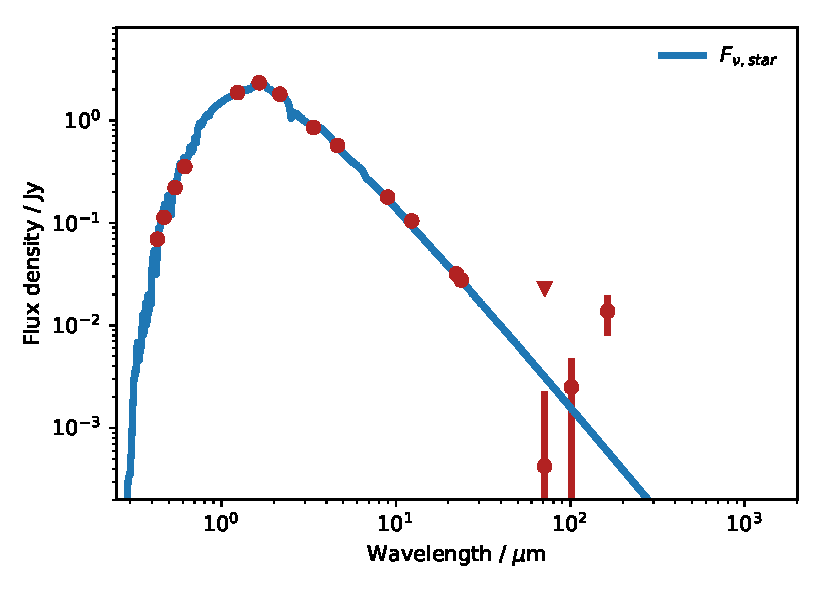
\includegraphics[width=\columnwidth]{sed_gj3305.pdf}
  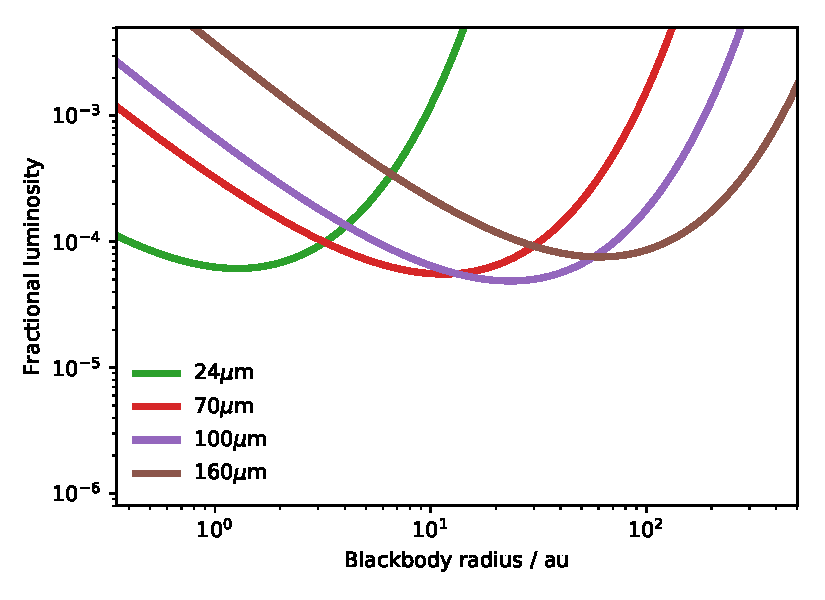
\includegraphics[width=\columnwidth]{f_r_gj3305.pdf}
  \caption{Spectrum and limits on dust emission around
    GJ~3305. (\emph{left panel}) Spectrum of the star (blue line) and
    photometry (dots and triangle). (\emph{right panel}) Limits on
    fractional luminosity as a function of blackbody dust radius, with
    the 3$\sigma$ detection limits that are achieved at 12, 24 and
    70$\mu$m.}
    \label{fig:gj3305}
\end{figure*}

Given an excess around 51~Eri itself, an obvious question is whether the
stellar companion, GJ~3305~AB
\citep{2001ApJ...562L..87Z,2006AJ....131.1730F}, shows a detectable
infrared excess. This binary was observed by Spitzer MIPS, WISE, and
\emph{Herschel} PACS, and shows no excess at any wavelength. A spectrum
from the \emph{Spitzer} InfraRed Spectrograph
\citep[IRS,][]{2004ApJS..154...18H,2011ApJS..196....8L} is consistent
with the stellar photosphere, though is not shown here. The spectrum and
limits are shown in Figure \ref{fig:gj3305}, with no disk above a
fractional luminosity of about $10^{-4}$. This lower sensitivity,
despite reasonably high quality photometry, illustrates the poorer
sensitivity to circumstellar dust around late-type stars that motivates
restricting the sample of directly imaged planet hosts to earlier types
when considering the possibility of planet-disk correlations.

\section{The directly imaged planet -- disk brightness
  correlation}\label{s:corr}

\begin{table*}
  \caption{Sample of systems with directly imaged planets hosted by A
    and F-type primaries. For HD~116434 the specific age derived by
    \citet{2017arXiv170701413C} is adopted. Spectral types are from Simbad.}\label{tab:pl}
  \begin{tabular}{llllll}
    \hline
    System & HD & Spec. type & Association & Age / Myr & Main age reference(s) \\
    \hline
    51 Eri & HD 29391 & F0 & $\beta$ Pictoris Moving Group & $24 \pm 3$ & \citet{2001ApJ...562L..87Z,2014MNRAS.445.2169M,2015MNRAS.454..593B} \\
    $\beta$ Pictoris & HD 39060 & A6 & $\beta$ Pictoris Moving Group & $24 \pm 3$ & \citet{2001ApJ...562L..87Z,2014MNRAS.445.2169M,2015MNRAS.454..593B} \\
    - & HD 95086 & A8 & Lower Centaurus Crux & $17 \pm 4$ & \citet{2013ApJ...775L..40M} \\
    - & HD 106906 & F5 & Lower Centaurus Crux & $17 \pm 4$ & \citet{2013ApJ...775L..40M} \\
    - & HD 116434 & A2 & Lower Centaurus Crux & $14 \pm 4$ & \citet{2017arXiv170701413C} \\
    Fomalhaut & HD 216956 & A4 & - & $440 \pm 40$ & \citet{1997ApJ...475..313B,2012ApJ...754L..20M} \\
    HR~8799 & HD 218396 & F0 & Columba & $42 \pm 5$ & \citet{2008hsf2.book..757T,2011ApJ...732...61Z,2015MNRAS.454..593B} \\
    \hline
  \end{tabular}
\end{table*}

We now briefly consider a sample comprising the systems with directly
imaged planets hosted by A and F-type primaries. This subset restricts
the systems to those listed in Table \ref{tab:pl}, which gives spectral
types from Simbad, and the current best age estimates and a few relevant
references. For a complete list and in-depth review of planet imaging,
the reader is referred to \citet{2016PASP..128j2001B}. As noted earlier,
HD~131399 is excluded from this list as the nature of the companion is
currently unclear \citep{2016Sci...353..673W,2017arXiv170506851N}, while
an alternative reason to exclude it could be the ($\sim$300au) proximity
of the companion HD~131399~BC, which could strongly influence the
evolution of the system in a way that makes it different to the other
systems considered.

HD~131399 illustrates that how this ``sample'' is defined is in part
arbitrary, since for example Fomalhaut~b might also be excluded, for the
sample to include only young ($\lesssim$100Myr-old) systems or those
that look like ``normal'' gas-giant planets
\citep[see][]{2008Sci...322.1345K,
  2011MNRAS.412.2137K,2013ApJ...775...56K}, and HD~106906~b might also
be excluded if only planets with projected separations within 100au are
considered. As in the HD~131399 system, the presence of other stellar
system components may also be important, thought both 51~Eri and
Fomalhaut are also multiple systems, albeit with wider separations. A
similar number of imaged planet systems with late-type primaries are
known \citep[e.g. 2MASS J12073346-3932539,][]{2004A&A...425L..29C}, but
these are not considered here because the sensitivity to circumstellar
dust around cool stars is much poorer than for A/F-type stars (see
Figure \ref{fig:gj3305}).

Given our chosen sample of directly imaged planet systems, and the
possibility of a perfect current record of 7/7 with detected thermal
debris disk emission, the question of whether a trend similar to that
seen for radial velocity planet hosts arises.

To test for a correlation requires a control sample of similar stars,
for which we use the sample of 119 Scorpius-Centaurus A-type stars
(those cooler than 9700K) in Upper Centaurus Lupus (UCL) and Lower
Centaurus Crux (LCC) from \citet{2012ApJ...756..133C}. A population of
lower mass stars could equally have been used, as the rate of infrared
excess detections is similar, but the fact that the F-type stars in
Table \ref{tab:pl} are no later than F5 suggests that a comparison with
A-types is more appropriate. The fraction of these stars with 24$\mu$m
excess detections and non-flagged 24$\mu$m photometry, given the
sensitivity limit of 1.12 derived in section \ref{s:hd116434:ss:det} is
$26/58 = 45\%$. A Fisher's exact test yields a two-tailed $p$-value of
0.01. The $p-$value is 0.005 if the number of control stars is doubled
at the same excess detection frequency, so while greater numbers are
clearly needed among the planet-host systems, having $>$100 stars in the
control sample is also important for the significance of such hypothesis
tests. When A-types with flagged 24$\mu$m photometry are included the
fraction is $43/119 = 36\%$, with a $p$-value of 0.001. These tests
therefore show that, at least naively, and depending on the control
sample used, there is evidence at
$\sim$$2-3\sigma$ for a correlation between directly imaged planets and
the brightness of debris disks in those systems.

While these hypothesis tests provide some evidence for a positive
correlation, there is a major caveat; many of the directly imaged
planets reside in systems that were targeted explicitly because they
were known to have infrared excesses
\citep[e.g. HD~95086,][]{2013A&A...553A..60R,2013ApJ...772L..15R}. This
bias means that the evidence discussed above can only be considered
circumstantial and not statistically significant. A sample of systems
that is unbiased with respect to the presence of infrared excesses is
needed for a proper hypothesis test. Such a sample could likely be
constructed at the completion of the GPI/GPIES and SPHERE/SHINE
Guaranteed Time direct imaging surveys, as long as the majority of stars
in nearby moving groups where planets have been found are observed
(e.g. to incorporate the currently discovered planets, all A/F stars in
the $\beta$ Pictoris moving group, Columba association, Lower Centaurus
Crux, and if Fomalhaut is considered, some representative sample of
nearby stars).

\section{Conclusions}\label{s:conc}

This work is motivated by the possible future detection of a correlation
between debris disk brightness and directly imaged planet
detection. With only a handful of imaged planets, such a correlation
requires careful consideration of the infrared excesses towards each
system. The systems HD~116434 and 51~Eri, both host to relatively faint
infrared excesses, were therefore revisited in order to gauge the
significance of HD~116434's excess, and consider the probable
architecture of these systems.

Through a careful analysis of a population of B/A-type stars observed
with Spitzer, the significance of the 24$\mu$m excess towards HD~116434
is quantified, and found to be at a level sufficient to claim a
detection. The level of significance is however relatively low, at
4$\sigma$, so given the anticipated high level of interest in this
system merits confirmation. Assuming the blackbody emission properties
typical of circumstellar dust, the excess is found to be relatively
warm, and incompatible with temperatures that would place the dust
exterior to the planet, which is currently at a projected separation of
92au. However, given the high rate of stellar rotation, an alternative
interpretation is that the emission originates from Be star-like
free-free emission in a stellar wind. This hypothesis is readily
testable with new mm-wave observations.

The properties of the disk orbiting 51~Eri are also considered. While
the significance or origin of the excess is not in doubt, previous works
came to apparently conflicting conclusions, so the aim here is to
reconcile these works. While the location of the disk around 51~Eri is
not certain, the tendency for small disks to evolve rapidly to
undetectable levels, and for imaged disks to be larger than blackbody
assumptions predict, mean that it is likely that the disk orbits
exterior to the planet.

Naively, the fact that the 7/7 A/F-type systems with directly imaged
planets may all host detected debris disks leads to the conclusion of a
$2-3\sigma$ significant positive correlation compared to a control
sample. However, some of the systems where directly imaged planets were
discovered were targeted specifically because they were known to host
debris disks. Any correlation therefore becomes less significant, and
therefore awaits results that can be derived from unbiased samples.

\section*{Acknowledgements}

GMK is supported by the Royal Society as a Royal Society University
Research Fellow.

This research has made use of the NASA/ IPAC Infrared Science Archive,
which is operated by the Jet Propulsion Laboratory, California Institute
of Technology, under contract with the National Aeronautics and Space
Administration, NASA's Astrophysics Data System Bibliographic Services,
the SIMBAD database and the VizieR catalogue access tool, operated at
CDS, Strasbourg, France
\citep{2000A&AS..143....9W,2000A&AS..143...23O}.

This work also benefited from the software \texttt{astropy}
\citep{2013A&A...558A..33A}, \texttt{bokeh} \citep{bokeh},
\texttt{emcee} and \texttt{corner} \citep{2013PASP..125..306F,corner},
\texttt{matplotlib} \citep{Hunter:2007}, \texttt{multinest} and
\texttt{pymultinest} \citep{2009MNRAS.398.1601F,2014A&A...564A.125B},
and \texttt{numpy} and \texttt{scipy} \citep{numpy2011}.

%%%%%%%%%%%%%%%%%%%%%%%%%%%%%%%%%%%%%%%%%%%%%%%%%%

%%%%%%%%%%%%%%%%%%%% REFERENCES %%%%%%%%%%%%%%%%%%

% The best way to enter references is to use BibTeX:

\bibliographystyle{mnras}
\bibliography{../ref} % if your bibtex file is called example.bib

%%%%%%%%%%%%%%%%%%%%%%%%%%%%%%%%%%%%%%%%%%%%%%%%%%

%%%%%%%%%%%%%%%%% APPENDICES %%%%%%%%%%%%%%%%%%%%%

\appendix

\section{Photometry and SED fitting}

The analysis of photometry for the target stars in this work is done
using two related sets of software, \texttt{sdb} and \texttt{sdf}. These
remain under development; it is likely that \texttt{sdb} will be
re-imagined completely to deal with larger samples, and parts of
\texttt{sdf} that produce web-based output for public and collaborative
access are a current focus.

The core of synthetic photometry and model fitting is very similar to a
previous \texttt{IDL} version developed for the Herschel DEBRIS survey
\citep[e.g.][]{2014MNRAS.445.2558T} and used for various other studies
\citep[e.g.][]{2012MNRAS.426...91K,2014MNRAS.444.3164K}. The current
\texttt{python} code is robust enough to produce consistent and reliable
results, as illustrated by the precision of the 24$\mu$m photometric
predictions in Figure \ref{fig:r}. Both packages are available
online\footnote{\href{www.github.com/drmk}{www.github.com/drgmk}},
though only \texttt{sdf} is expected to be particularly useful to
others. Interested users are encouraged to contact the author directly.

\texttt{sdb} (``star database'') uses a combination of
\texttt{vizquery}\footnote{\href{http://cdsarc.u-strasbg.fr/doc/vizquery.htx}{http://cdsarc.u-strasbg.fr/doc/vizquery.htx}},
\texttt{stilts} \citep{2006ASPC..351..666T}, url-based queries, shell
scripts, and a MySQL database to import information for a star of
interest from Simbad, and tables hosted by Vizier and the NASA/IPAC
Infrared Science Archive (IRSA). The primary information is photometry,
but other pertinent details, such as cross-identifier lists and spectral
types (Simbad) and positions, proper motions, and parallaxes
\citep{2007A&A...474..653V,2016A&A...595A...4L} are also collected.

Nearly 100 literature sources are searched for photometry for a given
target, large uniform catalogues are preferred as they allow internal
consistency checks such as that performed in section
\ref{s:hd116434:ss:det}, but inevitably smaller catalogues, and
individual measurements from single publications, must also be used. In
particular, a list of mm-wave photometry is part of the \texttt{sdb}
package, and is updated semi-regularly. The large catalogues that are
used are listed in Table \ref{tab:phot}, sorted in approximate order of
wavelength and separated into UV, optical, infrared, and (sub-)mm
sections.

% select concat(
% cat_name,' & ',
% ifnull(group_concat(band_name),''),' & ',
% ifnull(concat('[',group_concat(band),']'),''),' & ',
% concat('\\citet{',replace(bibcode,'\'',''),'}'),' ','\\\\') from xmatch where incl=1 group by cat_name
\begin{table*}
  \caption{Major photometric catalogues in \texttt{sdb}.}\label{tab:phot}
  \begin{tabular}{llll}
    \hline
    Catalogue name & Filter names & Filter wavelengths & Reference \\
    \hline
    GALEX DR5 & NUV,FUV & & {\citet{2011Ap&SS.335..161B}} \\
    \hline
    Tycho Double Star & $B_T$,$V_T$ &  & {\citet{2002A&A...384..180F}} \\
    Tycho-2 & $B_T$,$V_T$ &  & {\citet{2000A&A...355L..27H}} \\
    Heritage Stromgren & $b-y$,$c_1$,$m_1$ & & {\citet{2015A&A...580A..23P}} \\
    Heritage UBV & $U-B$,$B-V$,$V$ &  & \citet{2006yCat.2168....0M} \\
    APASS DR9 & $B$,$V$,$g$,$r$,$i$ & & \citet{2015AAS...22533616H} \\
    Hipparcos & $H_p$ & & \citet{1997ESASP1200.....P} \\
    DENIS (2005) & $i$ & & \citet{2005yCat....102002D} \\
    2MASS PSC & $J$,$H$,$K_s$ & & \citet{2003tmc..book.....C} \\
    \hline
    AKARI IRC V1.0 & S9W,S18W & 9 and 18$\mu$m,  & {\citet{2010A&A...514A...1I}} \\
    ALLWISE & W1,W2,W3,W4 & 3.4, 4.6, 12, and 22$\mu$m & \citet{2010AJ....140.1868W} \\
    SEIP &  & 3.6, 4.5, 5.8, 8, and 24$\mu$m & \href{http://irsa.ipac.caltech.edu/data/SPITZER/Enhanced/SEIP/overview.html}{IRSA} \\
    Herschel Archive &  & 70, 100, and 160$\mu$m & GMK (using method from DEBRIS) \\
    Herschel DEBRIS &  & 70, 100, 160, 250, 350, and 500$\mu$m & DEBRIS \citep[e.g.][]{2014MNRAS.445.2558T} \\
    Herschel PACS PSC &  &  70, 100, and 160$\mu$m & \citet{2017arXiv170505693M} \\
    Herschel PACS XSC &  & 70, 100, and 160$\mu$m  & \citet{2017arXiv170505693M} \\
    Herschel SPIRE PSC &  & 250, 350, and 500$\mu$m & Schulz et al. (2017) \\
    IRAS FSC &  & 12, 25, 60, and 100$\mu$m & \citet{1990IRASF.C......0M} \\
    IRAS PSC &  & 12, 25, 60, and 100$\mu$m & \citet{1988iras....1.....B} \\
    Spitzer FEPS &  & 70$\mu$m & \citet{2008ApJS..179..423C} \\
    Literature IR &  & various & various \\
    \hline
    JCMT SONS &  & 450 and 850$\mu$m & \citet{2017arXiv170601218H} \\
    Literature mm &  & various & various \\
    \hline
  \end{tabular}
\end{table*}

Many further catalogues and sources are used, most of which are to
collect as much MIPS 70$\mu$m photometry as possible: $B$, $V$, $R_C$,
and $I_C$ photometry from \citet{1990A&AS...83..357B}, $J$ and $K_s$
DENIS photometry of bright southern stars from
\citet{2004A&A...413.1037K}, $UBV$ photometry of bright southern stars
from \citet{2010MNRAS.403.1949K}, and MIPS 70$\mu$m photometry from
\citet{2006ApJ...652.1674B,2006ApJ...636.1098B,2009ApJ...705.1226B,2009ApJ...705.1646C,2012ApJ...756..133C,2014ApJS..211...25C,2013ApJ...768...25G,2007ApJ...667..527G,2010ApJ...710L..26K,2005ApJ...631.1170L,2011ApJS..193....4M,2009ApJ...699.1067M,2009ApJ...698.1068P,2008ApJ...681.1484R,2006ApJ...653..675S,2007ApJ...658.1289T,2008ApJ...674.1086T,2011ApJ...732...61Z}.

After data import, photometry sources can be exported to text files in
IPAC format, with metadata keywords containing additional information
(e.g. spectral type, coordinates, parallax). To keep track of their
origins, all data has an associated ADS bibcode.

Once data is exported, model fitting is done using the \texttt{python}
package dubbed \texttt{sdf} (``sed fitting''). The details of this
software will be presented elsewhere, but the method is largely similar
to other SED fitting packages that use synthetic photometry. Given a
grid of model spectra, synthetic photometry is first calculated in all
necessary filters \citep[see][for a primer]{2012PASP..124..140B}. For
this paper both stellar and disk models were necessary; the stellar
models were PHOENIX BT-Settl atmospheres using
\citet{2009ARA&A..47..481A} abundances, and the disk models were
``modified'' blackbodies (where the disk spectrum is a blackbody that is
multiplied by $\lambda^{-\beta}$ for $\lambda>\lambda_0$ to mimic the
poor grain absorption/emission efficiency at far-IR/mm wavelengths, thus
introducing two additional parameters).

For fitting, photometry from \texttt{sdb} is read in and converted to
fluxes using zero points derived from the CALSPEC Vega spectrum
\citep{2014AJ....147..127B}. Where necessary, small (percent level)
offsets have been applied to these zero points with the aim of bringing
all photometric systems into agreement for fitting across a population
of stars with a range of spectral types \citep[see][for descriptions of
this type of approach, here the bandpasses are not altered
however]{2000PASP..112..961B,2015PASP..127..102M}. With \texttt{sdf},
there remain inconsistencies among these systems, with a range of
probable causes, the three most important being incorrect filter
bandpasses, inconsistencies in zero point offsets derived from different
samples (some of which may be related to inaccurate fitting of surface
gravities), and missing opacity in the stellar models for cool
stars. However, because there is a significant body of near and
mid-infrared photometry, these issues are largely irrelevant for the
goal of precisely fitting stellar photosphere models with the goal of
comparison with 24$\mu$m photometry.

Minimisation to find the best fitting models uses \texttt{pymultinest}
\citep{2014A&A...564A.125B}, a \texttt{python} wrapper for
\texttt{multinest} \citep{2009MNRAS.398.1601F}, which is a software
package that efficiently samples the parameter space for a given
model. Because it samples the entire parameter space, it has the
advantage of being able to compute the Bayesian evidence for a given
model, which can be compared with the results from fitting alternative
models to decide which model should be preferred, including the penalty
incurred by models that have additional parameters. Thus, multiple
models can be fit to a given set of photometry (i.e. a star, and a
star+disk), and the evidence used to determine which model should be
preferred. An additional advantage is avoiding the need for reasonable
initial estimates prior to fitting.

The basic output from \texttt{sdf} is a set of best fit parameters,
which are then used to derive secondary parameters, such as stellar
radii and luminosities, and disk fractional luminosities. Using the
samples from \texttt{multinest}, or further MCMC fitting (e.g. with
\texttt{emcee}, as is done in this paper), posterior distributions for
all parameters can be obtained, and uncertainties in their values
estimated. The results can be plotted, output in web-based form using
the \texttt{bokeh} plotting library, or in image form using a package
such as \texttt{matplotlib}.

%%%%%%%%%%%%%%%%%%%%%%%%%%%%%%%%%%%%%%%%%%%%%%%%%%


% Don't change these lines
\bsp	% typesetting comment
\label{lastpage}
\end{document}

% End of mnras_template.tex